\section{Flots et coupes}
\subsection{Flots et coupes}
\index{flot}
\index{capacité}
\begin{mydef}
  Soit un graphe dirigé, dont les noeuds sont partitionnés en sources, puits et noeuds intermédiaires, et dont chaque arête $a$ porte un nombre réel $c(a)$ nommé \emph{capacité}.\\
  Un \emph{flot} est la donnée d'un nombre réel $f(a)$ sur chaque arête, tel que $0 \leq f(a) \leq c(a)$ et que le flot net sortant de chaque noeud intermédiaire soit nul.
\end{mydef}

\index{flot!flot net sortant}
\index{flot!valeur du flot}
\index{flot!flot maximum}
\begin{mydef}
  \begin{itemize}
    \item Le \emph{flot net sortant d'un noeud} $u$ est défini comme
      $\sum_{\text{arêtes }a\text{ d'origine }u} f(a) − \sum_{\text{arêtes }b\text{ de destination }u} f(b)$.
    \item Le \emph{flot net sortant d'un ensemble} $U$ de noeuds est la somme des flots nets sortant des noeuds de $U$.
    \item La \emph{valeur du flot} est le flot net sortant des noeuds sources.
  \end{itemize}
  On désire trouver le \emph{flot maximum}, c'est-à-dire le flot de valeur maximale.
\end{mydef}

\index{coupe}
\index{coupe!coupe minimum}
\begin{mydef}
  Une \emph{coupe} est un ensemble d'arêtes tel qu'il n'ait plus aucun chemin d'un noeud source vers un noeud puits quand on retire cet ensemble du graphe.\\
  On désire trouver une \emph{coupe minimum}, c'est-à-dire une coupe dont la capacité (i.e., la somme des capacités de ses arêtes) est minimale.
\end{mydef}

\begin{center}
  \begin{tikzpicture}
    \node[vertex] at (0, 0) (s) {\tiny $s$};
    \node[vertex] at (2, 1) (a) {\tiny $a$};
    \node[vertex] at (2, -1) (b) {\tiny $b$};
    \node[vertex] at (4, 1) (c) {\tiny $c$};
    \node[vertex] at (4, -1) (d) {\tiny $d$};
    \node[vertex] at (6, 0) (t) {\tiny $t$};
    \draw[->] (s) edge node[anchor = south] {\tiny $0 / 3$} (a);
    \draw[->] (s) edge node[anchor = north] {\tiny $0 / 2$} (b);
    \draw[->] (a) edge node[anchor = south] {\tiny $0 / 2$} (c);
    \draw[->] (a) edge node[anchor = south] {\tiny $0 / 3$} (d);
    \draw[->] (b) edge node[anchor = north] {\tiny $0 / 2$} (d);
    \draw[->] (c) edge node[anchor = south] {\tiny $0 / 2$} (t);
    \draw[->] (d) edge node[anchor = north] {\tiny $0 / 2$} (t);
  \end{tikzpicture}
\end{center}

\begin{center}
  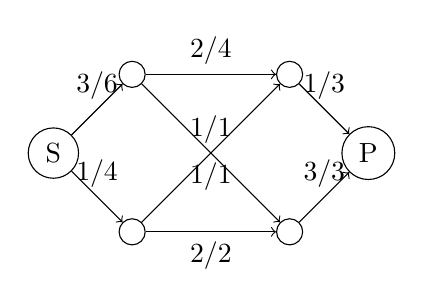
\begin{tikzpicture}
    \node[draw, circle] at (-2,0) (S) {S};
    \node[draw, circle] at (-1,1) (A) {};
    \node[draw, circle] at (-1,-1) (B) {};
    \node[draw, circle] at (1,1) (C) {};
    \node[draw, circle] at (1,-1) (D) {};
    \node[draw, circle] at (2,0) (P) {P};

    \draw[->] (S) edge node[anchor = south] {$3/6$} (A);
    \draw[->] (S) edge node[anchor = south] {$1/4$} (B);
    \draw[->] (A) edge node[anchor = south] {$2/4$} (C);
    \draw[->] (A) edge node[anchor = south] {$1/1$} (D);
    \draw[->] (B) edge node[anchor = north] {$1/1$} (C);
    \draw[->] (B) edge node[anchor = north] {$2/2$} (D);
    \draw[->] (C) edge node[anchor = south] {$1/3$} (P);
    \draw[->] (D) edge node[anchor = south] {$3/3$} (P);
  \end{tikzpicture}
\end{center}

\paragraph{Observation}
Se donner une coupe, on se donne un ensemble $S$ de noeuds atteignables à partir des sources,
c'est la même chose.
Lorsqu'on a une coupe, $S$ est la composante connexe comprenant les sources lorsqu'on enlève la coupe.
Lorsqu'on a $S$, la coupe est l'ensemble des arêtes reliant un noeud de $S$ et de $\bar{S}$.

\begin{mylem}
  Pour un flot donné, toutes les coupes ont le même flot net, qui est la valeur du flot.
  \begin{proof}
    Flot net de la coupe = Flot net(sources) + Flot net (s$\setminus$sources)
    =$f(S \to \bar{S}) - f(\bar{S} \to S)$
    taille de la coupe = capacité totale de la coupe
    \begin{center}
      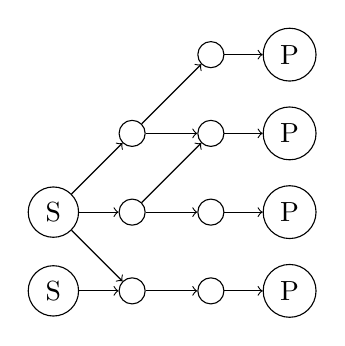
\begin{tikzpicture}
        \node[draw, circle] at (-2,0) (S1) {S};
        \node[draw, circle] at (-2,-1) (S2) {S};
        \node[draw, circle] at (-1,1) (A1) {};
        \node[draw, circle] at (-1,0) (A2) {};
        \node[draw, circle] at (-1,-1) (A3) {};
        \node[draw, circle] at (0,2) (B1) {};
        \node[draw, circle] at (0,1) (B2) {};
        \node[draw, circle] at (0,0) (B3) {};
        \node[draw, circle] at (0,-1) (B4) {};
        \node[draw, circle] at (1,2) (P1) {P};
        \node[draw, circle] at (1,1) (P2) {P};
        \node[draw, circle] at (1,0) (P3) {P};
        \node[draw, circle] at (1,-1) (P4) {P};

        \draw[->] (S1) edge (A1);
        \draw[->] (S1) edge (A2);
        \draw[->] (S1) edge (A3);
        \draw[->] (S2) edge (A3);
        \draw[->] (A1) edge (B1);
        \draw[->] (A1) edge (B2);
        \draw[->] (A2) edge (B2);
        \draw[->] (A2) edge (B3);
        \draw[->] (A3) edge (B4);
        \draw[->] (B1) edge (P1);
        \draw[->] (B2) edge (P2);
        \draw[->] (B3) edge (P3);
        \draw[->] (B4) edge (P4);
      \end{tikzpicture}
    \end{center}
  \end{proof}
\end{mylem}

\begin{mylem}
  Pour tout flot $f$ et toute coupe $S \to \bar{S}$,
  $\valeur(f) \leq \coupe(S \to \bar{S})$.
  L'égalité a lieu si et seulement si toutes les arêtes $a$ de la coupe $S \to \bar{S}$ sont $f$-saturées
  (i.e., $f(a) = c(a)$) et toutes les arêtes $b$ de $\bar{S} \to S$ sont $f$-nulles (i.e., $f(b) = 0$).

  \begin{proof}
    \begin{align*}
      \valeur(f) & = \text{flot sur la coupe}\\
             & = \sum \fnet(S \to \bar{S})\\
             & = \sum_{i \in S \atop {j \in \bar{S} \atop ij \in E}} f(ij) - \sum_{i \in S \atop {j \in \bar{S} \atop ji \in E}} f(ij)\\
             & \leq \sum_{i \in S \atop {j \in \bar{S} \atop ij \in E}} f(ij)\\
             & \leq \sum_{i \in S \atop {j \in \bar{S} \atop ij \in E}} c(ij)\\
             & = \coupe(S \to \bar{S}).
    \end{align*}
    Avec égalité si et seulement si $\sum_{i \in S\atop {j \in \bar{S}\atop ji \in E}} f(ij) = 0$ et
    $\sum_{i \in S\atop {j \in \bar{S}\atop ij \in E}} f(ij) = \sum_{i \in S\atop {j \in \bar{S}\atop ij \in E}} c(ij)$
    c'est à dire que toutes les arêtes qui lient un noeud de $S$ à un noeud de $\bar{S}$ sont saturées
    et que les arêtes qui lient un noeud de $\bar{S}$ à un noeud de $S$ ont un flot nul.
  \end{proof}
\end{mylem}

\begin{mycorr}
  Si un flot $f$ et une coupe $S\to\bar{S}$ sont tels que $\valeur(f) = \coupe(S\to\bar{S})$,
  alors ce flot est maximum et cette coupe minimum.
  \begin{proof}
    On vient de voir que dans le cas d'égalité, les arêtes étaient saturées et il n'y a aucun flot qui va de $\bar{S}$ à $S$
    Et donc ne peut plus faire passer de flot de $S$ à $\bar{S}$ ni par des arêtes directes (elles sont saturées),
    ni par des ``back edges'' (elles sont nulles car il n'y a pas de flot de $\bar{S}$ à $S$).

    Le fait que le flot est maximum et que la coupe est minimum est en fait simplement montré par la dualité.
    On sait que pour toute coupe $S\to\bar{S}$ et flot $f$, $\coupe(S\to\bar{S}) \geq \valeur(f)$.
    Dès lors, pour toute coupe $\coupe(S \to \bar{S}) \geq \flotmax$ et pour tout flot,
    $\coupemin \geq \valeur(f)$ et en particulier
    $\coupemin \geq \flotmax$.
    On a donc
    \[ \coupe(S \to \bar{S}) \geq \coupemin \geq \flotmax \geq \valeur(f) \]
    d'où $\coupe(S \to \bar{S}) = \coupemin$ et
    $\flotmax = \valeur(f)$ en cas d'égalité
    $\coupe(S \to \bar{S}) = \valeur(f)$.
  \end{proof}
\end{mycorr}

\index{chemin!chemin $f$-saturé}
\index{chemin!chemin $f$-augmentant}
\begin{mydef}
  Etant donné un flot $f$, à tout chemin $P$ dans le graphe non-dirigé sous-jacent associons la quantité $i(P) = \min_{a \in P} i(a)$, où $i(a) = c(a) − f(a)$ pour les arêtes $a$ prises par $P$ dans le sens direct, et $i(a) = f (a)$ pour les arêtes a prises dans le sens inverse.\\
  Un chemin $P$ est \emph{$f$-saturé} si $i(P) = 0$. Il est \emph{$f$-augmentant} s'il est non saturé, part d'un noeud source et arrive à un noeud puits.
\end{mydef}

\begin{myexem}
  En partant du flot $f$ avec un chemin $f$-augmentant
  montré à la figure~\ref{fig:faug},
  on peut créer un nouveau flot $f'$ valide.
  L'arête déjà remplie à $3/4$ nous oblige à ce que le flot n'augmente que de 1,
  $\valeur(f') = \valeur(f) + 1$.
  Le flot est alors modifié le long de ce chemin comme montré
  à la figure~\ref{fig:fprime}.
  \begin{figure}[h!]
    \centering
    \begin{tikzpicture}
      \SetGraphUnit{2}
      \GraphInit[vstyle=Dijkstra]
      \SetUpEdge[style={->},
      labelstyle = {draw}]
      \Vertex{S}
      \NOEA(S){A}
      \SOEA(A){B}
      \NOEA(B){C}
      \SOEA(C){D}
      \NOEA(D){T}
      \Edge[label=$1/5$](S)(A)
      \Edge[label=$2/3$](B)(A)
      \Edge[label=$3/4$](B)(C)
      \Edge[label=$2/2$](D)(C)
      \Edge[label=$0/4$](D)(T)
    \end{tikzpicture}
    \caption{Chemin $f$-augmentant}
    \label{fig:faug}
  \end{figure}
  \begin{figure}[h!]
    \centering
    \begin{tikzpicture}
      \SetGraphUnit{2}
      \GraphInit[vstyle=Dijkstra]
      \SetUpEdge[style={->},
      labelstyle = {draw}]
      \Vertex{S}
      \NOEA(S){A}
      \SOEA(A){B}
      \NOEA(B){C}
      \SOEA(C){D}
      \NOEA(D){T}
      \Edge[label=$2/5$](S)(A)
      \Edge[label=$1/3$](B)(A)
      \Edge[label=$4/4$](B)(C)
      \Edge[label=$1/2$](D)(C)
      \Edge[label=$1/4$](D)(T)
    \end{tikzpicture}
    \caption{Chemin avec $f'$}
    \label{fig:fprime}
  \end{figure}
\end{myexem}

\begin{mytheo}
  Un flot est maximum si et seulement s'il ne contient pas de chemin $f$-augmentant.
  \begin{proof}
    \begin{itemize}
      \item[$\Rightarrow$] Si il existe un chemin augmentant, alors on peut améliorer strictement le flot.
      \item[$\Leftarrow$]
        Soit $f$ un flot qui ne contient pas de chemin $f$-augmentant.
        Soit $S$ l'ensemble des noeuds qu'on peut atteindre à partir de la source avec
        des chemins non $f$-saturés.
        $S$ ne contient aucun puits.
        Soit une arête de $S \to \bar{S}$, elle est $f$-saturée par construction de $S$,
        sinon la destination de l'arête serait dans $S$.
        Soit une arête de $\bar{S} \to S$, elle doit être $f$-nulle pour la même raison.
        \begin{figure}[h!]
          \centering
          \begin{tikzpicture}[x=2cm,y=1cm]
            \SetGraphUnit{1}
            \GraphInit[vstyle=Dijkstra]
            \SetUpEdge[style={->},
            labelstyle = {draw}]
            \Vertex{S}
            \NOEA(S){A}
            \SOEA(S){B}
            \EA(A){a}
            \EA(B){b}
            \SOEA(a){T}
            \Edge[label=$4/4$,color=red](A)(a)
            \Edge[label=$0/5$,color=red](b)(B)
            \AddVertexColor{blue}{S,A,B}
            \AddVertexColor{green}{a,b,T}
          \end{tikzpicture}
        \end{figure}
        Dès lors,
        \begin{align*}
          \coupe(S\to\bar{S}) & = \text{valeur du flot qui quitte }S\text{ vers }\bar{S}\\
                              & = \text{valeur du flot net entre }S\text{ et }\bar{S}\\
                              & = \valeur(f)
        \end{align*}
        Cette coupe est la coupe mininum et ce flot est le flot maximum.
        La preuve prouve aussi que du flot max on déduit une coupe min de même valeur.\\ D'où  $\rightarrow$ Max Flow = Min cut.
    \end{itemize}
  \end{proof}
\end{mytheo}

\begin{mytheo}
  La valeur du flot maximum et la capacité de la coupe minimum sont toujours égales.
  \begin{proof}
    Cette preuve n'a pas été vue au cours, on l'obtiens cependant facilement par contradiction.
  \end{proof}
\end{mytheo}

\subsection{L'algorithme de Ford-Fulkerson}
\index{algorithme!algorithme de Ford-Fulkerson}
\begin{myalgo}[Algorithme de Ford-Fulkerson]
  Algorithme \addTODO
\end{myalgo}


\begin{mylem}
  \label{lem:flot_chemin}
  Dans tout graphe dirigé avec un noeud source $u$ et un noeud puits $v$ et chaque arête de capacité un, le nombre maximum de chemins dirigés de u vers v disjoints deux à deux par les arêtes est la valeur du flot maximum.
  \begin{proof}
    Si j'ai $k$ chemins disjoints $u \to v$,
    je crée un flot de valeur $k$ en saturant les arêtes
    des chemins.
    \begin{figure}[h!]
      \centering
      \begin{tikzpicture}
        \SetGraphUnit{2}
        \GraphInit[vstyle=Dijkstra]
        \SetUpEdge[style={->},
        labelstyle = {draw}]
        \Vertex{S}
        \NOEA(S){A1}
        \EA(A1){A2}
        \SOEA(A2){T}
        \EA(S){B1}
        \EA(B1){B2}
        \EA(B2){T}
        \SOEA(S){C1}
        \EA(C1){C2}
        \NOEA(C2){T}
        \Edge[label=$1/1$](S)(A1)
        \Edge[label=$1/1$](A1)(A2)
        \Edge[label=$1/1$](A2)(T)
        \Edge[label=$1/1$](S)(B1)
        \Edge[label=$1/1$](B1)(B2)
        \Edge[label=$1/1$](B2)(T)
        \Edge[label=$1/1$](S)(C1)
        \Edge[label=$1/1$](C1)(C2)
        \Edge[label=$1/1$](C2)(T)
      \end{tikzpicture}
    \end{figure}
    $\flotmax \geq \#\{\text{chemins disjoints }u \to v\}$.

    De plus, considérons le flot max de $u \to v$.
    Partant d'un flot initial \emph{entier},
    Ford-Fulkerson le maintient \emph{entier},
    d'où il existe un flot maximum entier.

    Il existe donc un flot maximum binaire: 0 ou 1
    sur chaque arête.
    Prenons $E$, le nombre d'arêtes de flot 1.
    C'est un sous-graphe.
    Si ni source ni puits,
    degré entrant = degré sortant (sur $E$).
    Si $\flotmax = k$,
    il existe $k$ arêtes sortantes de $u$ dans $E$ que
    je peux prolonger par $k$ chemins (disjoints par les arêtes)
    vers $v$.

    \begin{figure}[h!]
      \centering
      \begin{tikzpicture}[x=2cm,y=1cm]
        \SetGraphUnit{1}
        \GraphInit[vstyle=Dijkstra]
        \SetUpEdge[style={->},
        labelstyle = {draw}]
        \SetVertexNoLabel
        \Vertex[NoLabel=false,L=$u$]{u}
        \NOEA(u){a}
        \SOEA(u){b}
        \SOEA(a){o}
        \NOEA(o){c}
        \SOEA(o){d}
        \SOEA[NoLabel=false,L=$v$](c){v}
        \Edges[color=blue](u,a,o,d,v)
        \Edges[color=green](u,b,o,c,v)
      \end{tikzpicture}
    \end{figure}
  \end{proof}
\end{mylem}

\begin{mytheo}
  \label{theo:kconnexe_chemin}
  Un graphe (non-dirigé) est $k$-arête-connexe si et seulement si entre toutes paires de noeuds il y a au moins $k$ chemins disjoints deux à deux par les arêtes.
  \begin{proof}
    \begin{itemize}
      \item[$\Leftarrow$]
        Si j'enlève $k-1$ arêtes quelconques
        entre $u$ et $v$, je coupe au plus $k-1$
        chemins des $k$ chemins disjoints.
        Il en reste au moins 1.
      \item[$\Rightarrow$]
        $k$-arête-connexe signifie que toute coupe entre $u$
        et $v$ a une capacité d'au moins $k$ (pour capacité 1
        sur les arêtes) car $\coupemin = k$.
        Le flot max de $u$ vers $v$ est donc $k$.
        Par le Lemme~\ref{lem:flot_chemin},
        il existe $k$ chemins disjoints par les arêtes de
        $u \to v$.
    \end{itemize}
  \end{proof}
\end{mytheo}

\begin{mytheo} [Menger]
  Un graphe (non-dirigé) est $k$-connexe si et seulement si entre chaque paire de noeuds il y a au moins $k$ chemins disjoints deux à deux par les noeuds.
  \begin{proof}
    Pour se ramener au théorème~\ref{theo:kconnexe_chemin},
    on va ``tranformer les noeuds en arêtes''.
    \begin{table}[h!]
      \centering
      \begin{tabular}{cc}
        Graphe non dirigé $G$ & Graphe dirigé $G'$\\
        \begin{tikzpicture}
          \SetGraphUnit{1}
          \GraphInit[vstyle=Dijkstra]
          \SetUpEdge[style={->}]
          \Vertex[L=$u$]{u}
        \end{tikzpicture}
        &
        \begin{tikzpicture}
          \SetGraphUnit{1}
          \GraphInit[vstyle=Dijkstra]
          \SetUpEdge[style={->}]
          \Vertex[L=$u_0$]{u0}
          \EA[L=$u_1$](u0){u1}
          \Edge(u0)(u1)
        \end{tikzpicture}\\
        \begin{tikzpicture}
          \SetGraphUnit{1}
          \GraphInit[vstyle=Dijkstra]
          \Vertex[L=$u$]{u}
          \SO[L=$v$](u){v}
          \Edge(u)(v)
        \end{tikzpicture}
        &
        \begin{tikzpicture}
          \SetGraphUnit{1}
          \GraphInit[vstyle=Dijkstra]
          \SetUpEdge[style={->}]
          \Vertex[L=$u_0$]{u0}
          \EA[L=$u_1$](u0){u1}
          \SO[L=$v_0$](u0){v0}
          \EA[L=$v_1$](v0){v1}
          \Edge(u0)(u1)
          \Edge(v0)(v1)
          \Edge(u1)(v0)
          \Edge(v1)(u0)
        \end{tikzpicture}\\
        \begin{tikzpicture}
          \SetGraphUnit{1}
          \GraphInit[vstyle=Dijkstra]
          \Vertex[L=$u$]{u}
          \SO[L=$v$](u){v}
          \SO[L=$w$](v){w}
          \Edge(u)(v)
          \Edge(v)(w)
        \end{tikzpicture}
        &
        \begin{tikzpicture}
          \SetGraphUnit{1}
          \GraphInit[vstyle=Dijkstra]
          \SetUpEdge[style={->}]
          \Vertex[L=$u_0$]{u0}
          \EA[L=$u_1$](u0){u1}
          \SO[L=$v_0$](u0){v0}
          \EA[L=$v_1$](v0){v1}
          \SO[L=$w_0$](v0){w0}
          \EA[L=$w_1$](w0){w1}
          \Edge(u0)(u1)
          \Edge(v0)(v1)
          \Edge(w0)(w1)
          \Edge(u1)(v0)
          \Edge(v1)(u0)
          \Edge(v1)(w0)
          \Edge(w1)(v0)
        \end{tikzpicture}\\
      \end{tabular}
    \end{table}[h!]
    $k$ chemins $u \to v$ disjoints par les noeuds
    $\rightarrow$ en $k$ chemins $u_0 \to v_1$ disjoints
    par les arêtes.
    Flot max $u \to v$ $\rightarrow$ Flot max de $u_0 \to v_1$
    de même valeur.

    $k$-connexe $\leftrightarrow$ en $k$-arête connexe.
    On applique le théorème~\ref{theo:kconnexe_chemin} sur $v'$,
    on en déduit le théorème de Menger sur $v$.
  \end{proof}
\end{mytheo}

